\section{Realization}
\label{sec:realization}
%Focus generale sulle tecnologie utilizzate
In this section, we outline the technical aspects concerning the realization of our solution. Therefore, we first present the enabler technologies through which we instantiate the design principles presented in \cref{sec:design}. After that, we discuss the CONFINE interaction protocol. Finally, we show the implementation details.

\subsection{Deployment}
As follows, we bridge the gap between the CONFINE high-level architecture and its practical realization. \cref{fig:deployment_diagram} depicts a \textit{UML deployment diagram} \cite{koch2002expressive} that aims to help with understanding the instantiated technologies. We differentiate between the technologies designated for mining, denoted as \Compo{Miner Node}s, and those specifically associated with provisioners, identified as \Compo{Provisioner Node}s. To enhance clarity, we maintain the separation of these \textit{devices} in the accompanying diagram. However, organizations have the flexibility to opt for integrated technologies that incorporate both mining and provisioning functionalities. Using our motivating scenario as an example, the \Actor{Hospital} can be equipped with machines aimed for both mining and provisioning, while the \Actor{Specialized clinic} can make use of separate devices. We included the \texttt{Log Recorder}, the \texttt{Log Provider}, and \texttt{Secure Miner} (already discussed in \cref{sec:design}) as abstract \textit{components} of the diagram, whose manifestations are described as follows. 

\Compo{Provisioner Node}s host \Compo{Provisioner}s components, encompassing the \Compo{Log Recorder} and \Compo{Log Provider}. 
We manifest the \Compo{Log Recorder} in the Process-Aware Information System (\Compo{PAIS}), which plays a crucial role in managing various business processes, including accounting and resource management \cite{Dumas.etal/2018:FundamentalsofBPM}. In our motivating scenario, the \Actor{Hospital} and the other provisioners generate Alice and Bob's traces through this class of systems.
\begin{figure}[t]
	\centering
	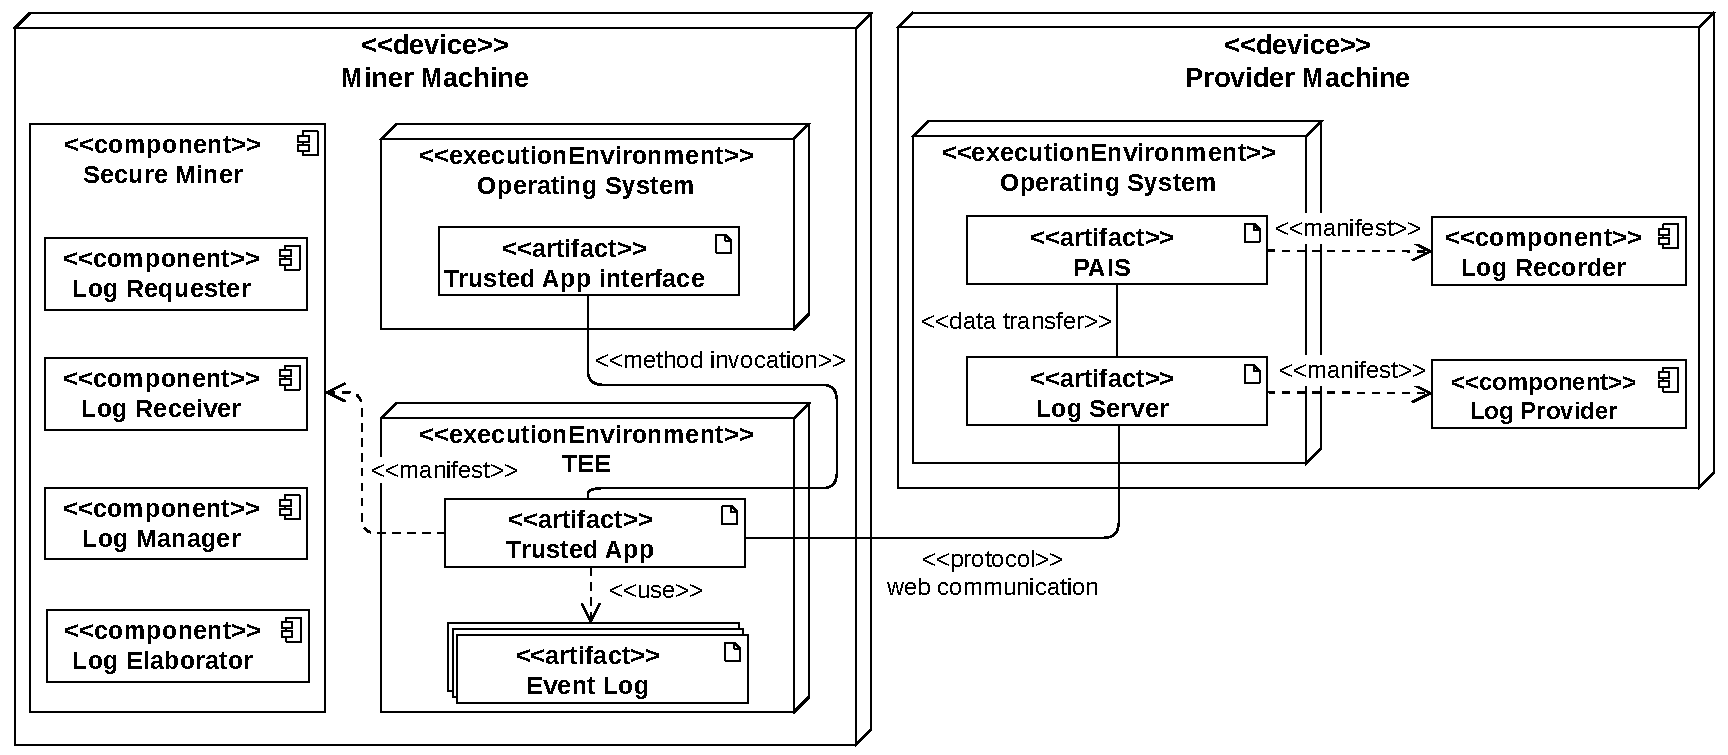
\includegraphics[width=1\linewidth]{content/figures/deploymentdiagram3.pdf}
	\caption{UML deployment diagram.}
	\label{fig:deployment_diagram}
\end{figure}
The \Compo{PAIS} grants access to the \Compo{Log Server}, enabling it to retrieve event logs. The \Compo{Log Server}, on the other hand, embodies the functionalities of the \Compo{Log Provider}, implementing web services aimed at handling remote data requests and providing event log data to miners. The \Actor{Hospital}, the \Actor{Specialized Clinic}, and the \Actor{Pharmaceutical Company} of our running example employes \Compo{Log Servers} adhering to established web standards such as HTTP\footnote{\url{w3.org/Protocols/rfc2616/rfc2616.html}. Accessed: \today.}, FTP\footnote{\url{w3.org/Protocols/rfc959/}. Accessed: \today.}, and Goopher\footnote{\url{datatracker.ietf.org/doc/html/rfc1436}. Accessed: \today.}. The \Compo{PAIS} and \Compo{Log Server} run on the top of the \Compo{Operating System} of the \Compo{Provisioner Node}.

The \Compo{Miner Node} is characterized by two distinct \textit{execution environments}: the \Compo{Operating System} and the Trusted Execution Environment (\Compo{TEE}). \Compo{TEE}s establish isolated contexts separate from the normal \Compo{Operating System}, safeguarding code and data through hardware-based encryption mechanisms. This technology relies on specialized components of the \Compo{Miner Node}'s CPU capable of handling encrypted data within a reserved section of RAM \cite{TEEHERE}. We leverage the security guarantees provided by \Compo{TEE}s to protect a \Compo{Trusted App} responsible for fulfilling the functions of the \Compo{Secure Miner} and its associated subcomponents. %The \Compo{Trusted App} consolidates the logic required for generating verifiable data requests, receiving external event logs, securely storing them within the \Compo{TEE}, and executing process mining algorithms. %All procedures executed by the \Compo{Trusted App} are tamper-proof. 
The \Compo{TEE} ensures the integrity of the \Compo{Trusted App} code, protecting it against malicious manipulations and unauthorized access by entities running within the \Compo{Operating System}. Additionally, we utilize the isolated environment of \Compo{TEE}s to securely store event log data (e.g., Alice and Bob's traces of our example) from provisioner organizations within the \Compo{Miner Node}. The \Compo{TEE} safeguards this sensitive information alongside a unique public and private key couple used for attestation purposes, preventing exposure to the \Compo{Operating System}. Access to data located in the \Compo{TEE} is restricted solely to the \Compo{Trusted App}. Users interact with the \Compo{Trusted App} through the \Compo{Trusted App Interface}, which serves as the exclusive communication channel. The \Compo{Trusted App} offers secure methods, invoked by the \Compo{Trusted App Interface}, for safely receiving information from the \Compo{Operating System} and outsourcing the results of computations, maintaining a high level of data security.

\begin{comment}
\begin{figure}[t]
\centering
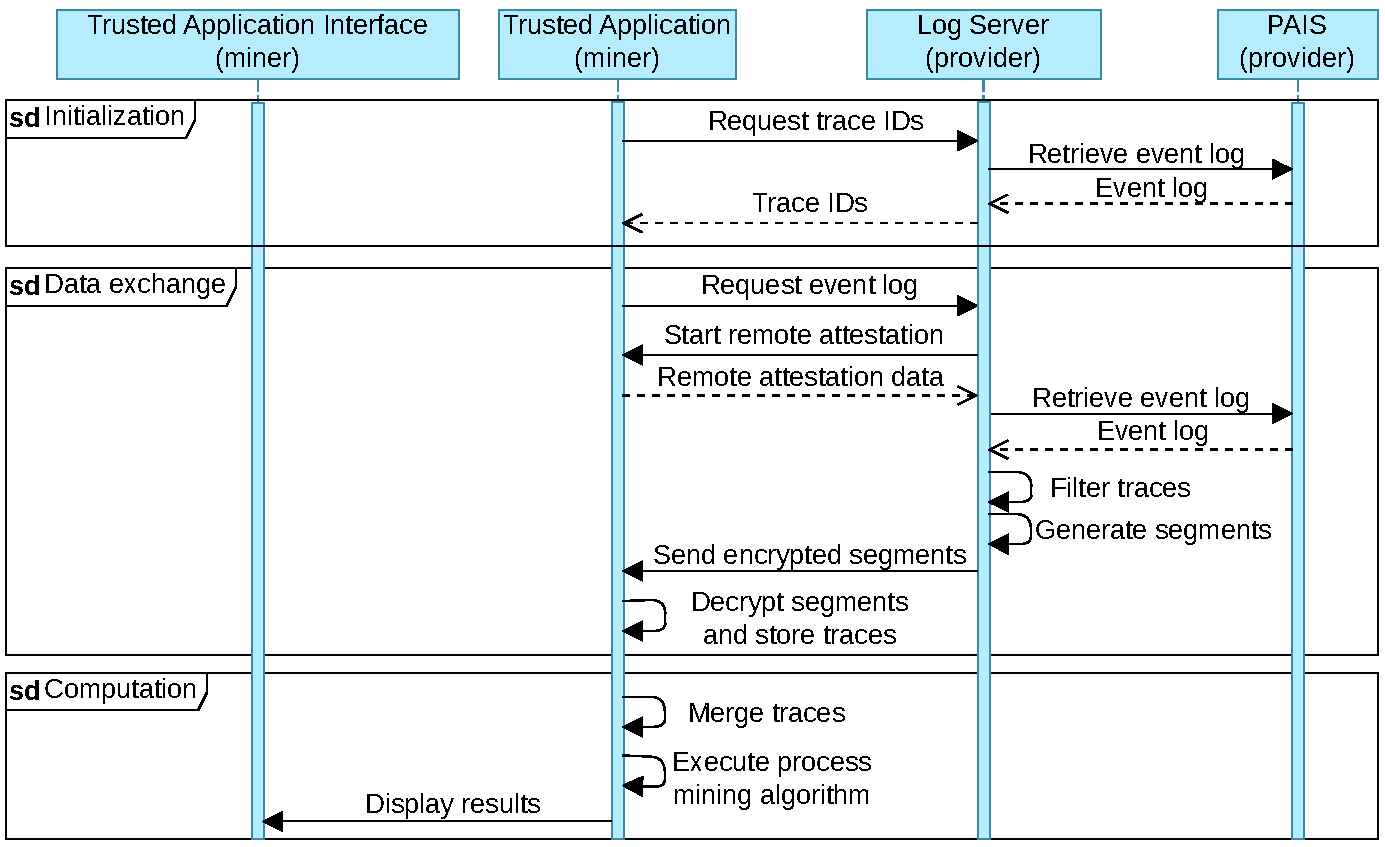
\includegraphics[width=0.9\linewidth]{content/figures/sequencediagram.pdf}
\caption{UML sequence diagram.}
\label{fig:sequence_diagram}
\end{figure}
\end{comment}


\subsection{CONFINE protocol}

We separate the protocol into subsequent stages, namely \textit{initialization}, \textit{remote attestation}, \textit{data transmission}, and \textit{computation}. This sequence of phases is enacted by two principal entities: a \Compo{Miner Node} and a variable number, denoted in as \texttt{n}, of \Compo{Provisioner Nodes}. We depict each stage in \cref{fig:workflow} and \cref{fig:workflow2}.

\begin{figure}[t]
	\subfloat[][Initialization]{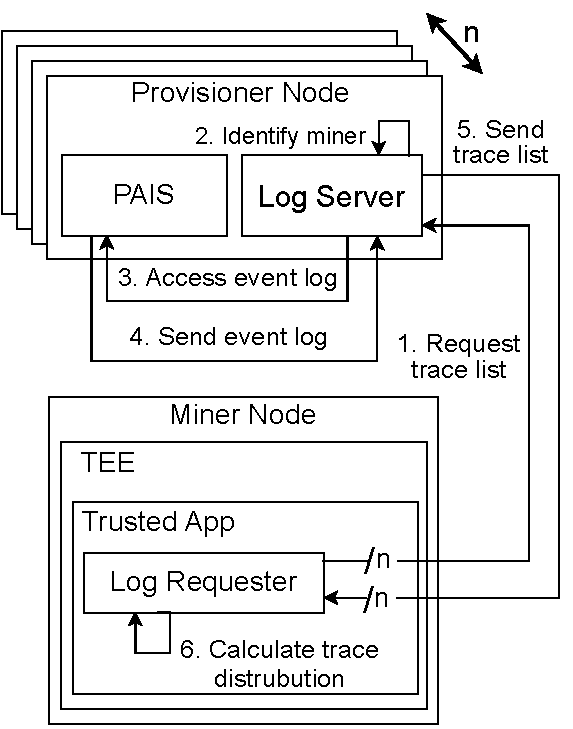
\includegraphics[width=0.29\linewidth]{content/figures/initializationworkflow.pdf}\label{fig:init}}\hfill
	\subfloat[][Remote Attestation]{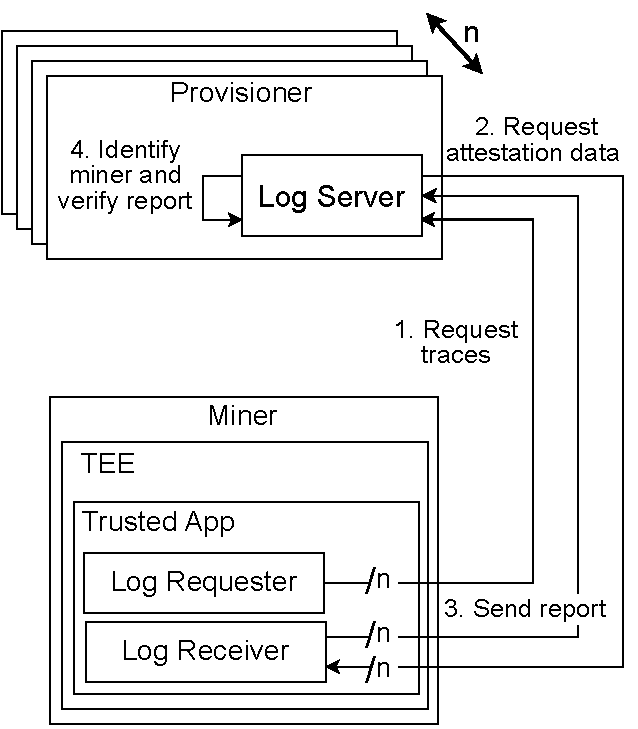
\includegraphics[width=0.32\linewidth]{content/figures/attestationworkflow.pdf}\label{fig:attestation}}\hfill
	\subfloat[][Data Transmission]{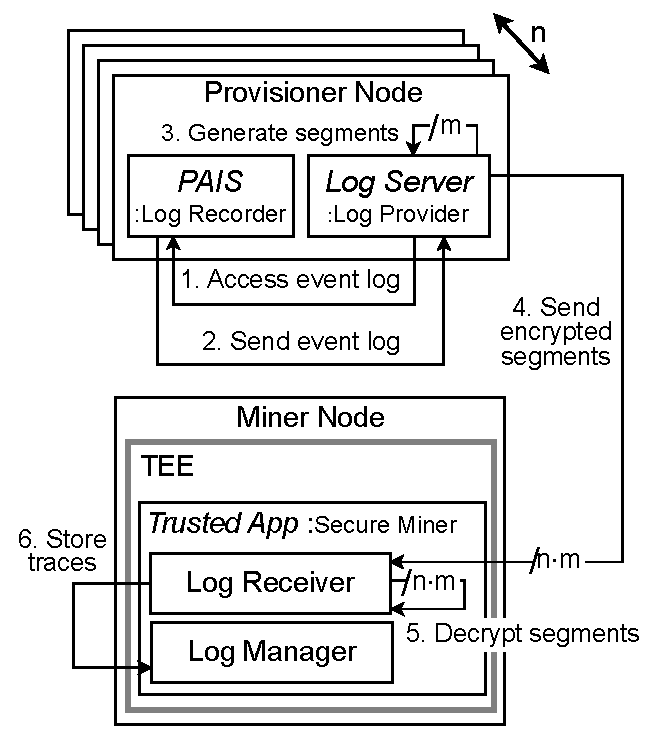
\includegraphics[width=0.33\linewidth]{content/figures/datatransmissionworkflow.pdf}\label{fig:transmission}}\hfill
	\caption{Initialization, remote attestation and data transmission phases of the CONFINE protocol.}
	\label{fig:workflow}
\end{figure}
\textbf{Initialization.} The objective of the initialization stage is to inform the miner about the distribution of traces related to a business process among the \Compo{Provisioner Nodes}. At the onset of this stage, the \Compo{Log Requester} component within the \Compo{Trusted App} issues \texttt{n} requests to the \Compo{Log Server} components of the provisioners for the list of owned traces (\texttt{1}, in \cref{fig:init}). Following sender authentication (\texttt{2}), each \Compo{Log Server} retrieves the local event log from the \Compo{PAIS} (\texttt{3}, \texttt{4}) and subsequently responds to the \Compo{Log Requester} by providing a list of its associated traces (5). After collecting these \Compo{n} responses, the \Compo{Log Requester} delineates the distribution of traces. In the context of our motivating scenario, by the conclusion of the initialization phase, the miner gains knowledge that traces belonging to Bob's process, specifically $T^H_{711}$ and $T^C_{711}$, are exclusively retained by the \Actor{Hospital} and the \Actor{Specialized Clinic}. In contrast, traces recording the Alice's process, denoted as $T^H_{312}$, $T^C_{312}$, and $T^S_{312}$, are scattered across all three organizations.

\textbf{Remote Attestation.} The remote attestation serves the purpose of establishing trust between miners and provisioners in the context of fulfilling data requests. This phase adheres to the overarching principles outlined in the RATS RFC standard~\cite{rfc9334} serving as the foundation for several attestation schemes (e.g., Intel EPID,\footnote{\url{sgx101.gitbook.io/sgx101/sgx-bootstrap/attestation}. Accessed: \today.} and AMD SEV-SNP\footnote{\url{amd.com/en/processors/amd-secure-encrypted-virtualization}. Accessed: \today.}). Remote attestation has a dual objective: (i) to furnish provisioners with compelling evidence that the data request for an event log originates from a \Compo{Trusted App} executing within a \Compo{TEE}, and (ii) to confirm the precise nature of the \Compo{Trusted App} as an authentic \Compo{Secure Miner} software entity. Upon the initiation of a new log request by the \Compo{Log Requester} (\texttt{1}, in \cref{fig:attestation}), each of the \texttt{n} \Compo{Log Server}s commences the verification process by requesting the necessary information from the \Compo{Log Receiver} to conduct the attestation (\texttt{2}). Subsequently, the \Compo{Log Receiver} generates the attestation report containing the measurement of the \Compo{Trusted App}, which is defined as the hash value of the combination of the code and initial data of the \Compo{Secure Miner}. Once this report is signed using the attestation private key associated with the hardware of the \Compo{Miner Node}, it is transmitted by the \Compo{Log Receiver} to the \Compo{Log Server}s alongside the attestation public key of the \Compo{Miner Node} (\texttt{3}). The \Compo{Log Server}s authenticate the miner using the public key and decrypt the report (\texttt{4}). In this last step, the \Compo{Log Server}s undertake a comparison procedure in which they juxtapose the measurement found within the decrypted report against a predefined reference value associated with the source code of the \Compo{Secure Miner}. If the decrypted measurement matches the predefined value, the \Compo{Miner Node} gains trust from the provisioned.

\begin{wrapfigure}[12]{r}{0.4\textwidth}
	\vspace{-2em}
	%\centering
	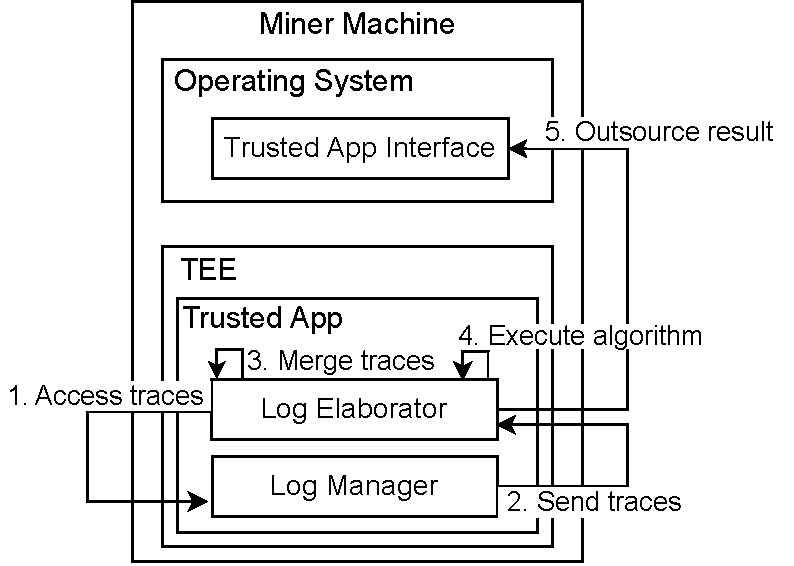
\includegraphics[width=1\textwidth]{content/figures/computationworkflow.pdf}
	\caption[A gull]{Computation phase of the CONFINE protocol.}
	\vspace{-2pt}
	\label{fig:workflow2}
\end{wrapfigure}
\textbf{Data Transmission.} Once verified the trusted nature of the \Compo{Trusted App}, the \Compo{Log Servers} proceed with the transmission of their traces. To accomplish this, each \Compo{Log Server} retrieves the event log from the \Compo{PAIS} (\texttt{1} and \texttt{2}, in \cref{fig:transmission}), and divides it into segments, resulting in \texttt{m} segments (\texttt{3}). Each of these segments contains a variable number of complete traces, with the cumulative size remaining within the threshold specified by the miner as a parameter of the initial request. As an illustrative example from our motivating scenario, the \Compo{Log Server} of the \Actor{Hospital} may structure the segmentation such that $T^H_{312}$ and $T^H_{711}$ reside within the same segment, whereas the \Actor{Specialized clinic} might have $T^S_{312}$ and $T^S_{711}$ in separate segments. Subsequently, the \texttt{n} \Compo{Log Server}s transmit their \texttt{m} encrypted segments to the \Compo{Log Receiver} of the \Compo{Trusted App} (\texttt{4}). The \Compo{Log Receiver}, in turn, decrypts each of the \texttt{n} • \texttt{m} responses (\texttt{5}) and securely stores the traces within the \Compo{TEE} through the \Compo{Log Manager} (\texttt{6}).

\textbf{Computation.} The \texttt{Trusted App} requires all the provisioners to have delivered traces referring to the same process instances. For example, when $T^H_{312}$, $T^S_{312}$ and $T^C_{312}$ have all been received by the \Compo{Trusted App}, the process instance associated with Alice becomes eligible for computation. The computation procedure may be activated either manually by the user operating the \Compo{Miner Node} or automatically upon the fulfillment of predetermined conditions (e.g., as soon as all the traces are collected). Upon meeting these conditions, the \Compo{Log Elaborator} requests the traces earmarked for computation from the \Compo{Log Manager} (\texttt{1} and \texttt{2}, in \cref{fig:workflow2}). To reconstruct a complete process instance traces belonging to the same process instance must be merged by the \Compo{Log Elaborator} in a single trace (e.g., $T_{312}$ for Alice case) comprehensive of all the events in the partial traces (e.g., $T^H_{312}$, $T^S_{312}$ and $T^C_{312}$ for Alice case). To accomplish this, the \Compo{Log Elaborator} applies a specific \textit{merging schema} as stated in \cite{claes2014merging}. According to this research work, a merging schema is defined as a rule specifying the attributes that link two traces during the merging process. In our illustrative scenario, the traces of Alice and Bob are related by the same case id (i.e., 312 for Alice case, and 711 for Bob case). Therefore, the merging schema to combine their traces is contingent upon the linkage established by the \texttt{concept:name} attribute, as exemplified below:
\begin{lstlisting}[numbers=none]
    merge all traces where
    	"concept:name" of trace in log A
    				equals
    	"concept:name" of trace in log B
\end{lstlisting}
We underline that our solution allows for various merging schemas involving different trace attributes. After the merging operation (\texttt{3}), the \Compo{Log Elaborator} proceeds to input the merged traces into the process mining algorithm (\texttt{4}). Ultimately, the outcome of the computation is relayed by the \Compo{Log Elaborator} from the \Compo{TEE} to the \Compo{Trusted App Interface} running atop the \Compo{Operating System} of the \Compo{Miner Node} (\texttt{5}).

\subsection{Implementation}
\label{sec:implementation:details}
We implemented the \texttt{Secure Miner} component as an Intel SGX\footnote{\url{sgx101.gitbook.io/sgx101/}. Accessed: \today.} trusted application, encoded in Go through the EGo framework.\footnote{\url{docs.edgeless.systems/ego}. Accessed: \today.} To demonstrate the effectiveness of our framework, we integrated the \textit{HeuristicsMiner} discovery algorithm within the \Compo{Trusted Application}. We established the communication between miners and provisioners using the HTTP web protocol. Upon successful execution, our \textit{HeuristicsMiner} implementation generates workflow nets corresponding to the analyzed processes. For additional details, our implementation can be accessed publicly at the following url: \url{github.com/dave0909/TEExProcessMining/}.
